\documentclass[12pt,a4paper]{article}
\usepackage[a4paper,margin=2.54cm]{geometry}
\usepackage[T1]{fontenc}
\usepackage{mathptmx}
\usepackage[american]{babel}
\usepackage{csquotes}
\usepackage[style=apa,backend=biber]{biblatex}
\addbibresource{references.bib}
\usepackage{amsmath}
\usepackage{siunitx}
\usepackage{graphicx}
\usepackage{booktabs}
\usepackage{setspace}
\usepackage{enumitem}
\usepackage[framemethod=default]{mdframed}
\usepackage{titlesec}
\usepackage{fancyhdr}
\usepackage[labelfont=bf,labelsep=newline,textfont=it,justification=raggedright,singlelinecheck=false,skip=2pt,font=normalsize]{caption}
\usepackage[hidelinks]{hyperref}
\usepackage{xcolor}
\hypersetup{urlcolor=blue!60!black,colorlinks=true,linkcolor=black,citecolor=black}
\sisetup{separate-uncertainty=true,mode=math}
\DeclareSIUnit\ohm{\ensuremath{\Omega}}
\setstretch{1.08}
\setlength{\parindent}{0.5in}
\setlength{\parskip}{0pt}
\setlist{nosep,leftmargin=0.5in}
\titleformat{\section}{\centering\bfseries\large}{}{0pt}{}
\titleformat{\subsection}{\centering\bfseries}{}{0pt}{}
\titlespacing*{\section}{0pt}{14pt}{6pt}
\titlespacing*{\subsection}{0pt}{12pt}{4pt}
\pagestyle{fancy}\fancyhf{}\fancyhead[R]{\thepage}\renewcommand{\headrulewidth}{0pt}
\fancypagestyle{plain}{\fancyhf{}\renewcommand{\headrulewidth}{0pt}}
\newcommand{\figurenote}[1]{\par\vspace{2pt}{\small\raggedright\noindent\textit{Note.} #1\par}}
\newcommand{\todo}[1]{}
\DeclareCaptionLabelFormat{appendix}{#1 A#2}
\begin{document}
\thispagestyle{plain}
\begin{center}
{\Large\bfseries No Current, No Braking: Two Instrument Lessons From a Magnet--Coil Damping Experiment\par}
\vspace{8pt}\rule{\linewidth}{0.4pt}\vspace{2pt}

\textit{Hassan Tariq Malik, Hardyesh Kumar, and Muhammad Umer Farooq}\\
\textit{The Black Hole Science Lab, Islamabad, Pakistan}\\
{\small Research supervisors: M. Sanan Qureshi (The Black Hole), Dr Sadia Manzoor (COMSATS University Islamabad), and Dr Pervez Hoodbhoy (The Black Hole)}\\[1pt]
{\small ORCID (H.\,T.\,Malik): \href{https://orcid.org/0009-0001-3749-090X}{0009-0001-3749-090X} \;\textperiodcentered\; Correspondence: \href{mailto:hassantariq102938@gmail.com}{hassantariq102938@gmail.com}}
\end{center}
\vspace{-2pt}
{\setstretch{1.0}\noindent\textbf{Abstract.} A magnet oscillating on a spring above a coil is a standard demonstration of electromagnetic braking, usually checked by showing that the damping scales as $1/R$ with the resistance of the coil circuit. We attempted this check with a US\$43 data-acquisition system built around a Raspberry Pi Pico. Across series resistances from \SI{15}{\ohm} to \SI{2.2}{\mega\ohm} the decay rate did not change: $\gamma = (11.9 \pm 0.5)\times10^{-3}\,\mathrm{s^{-1}}$ ($n = 8$). The coil was closed only through the amplifier's \SI{1}{\mega\ohm} bias resistor, so the braking current was about \SI{16}{nA} and the electromagnetic damping a few millionths of the total. For spring~1, a loop closed through the coil alone would have added about 17\%, which the data disfavour at 2.3--3 standard deviations, depending on the assumed amplitude. A second hidden error was the clock: mains hum recorded at \SI{63}{Hz} instead of \SI{50}{Hz} showed that each stored sample took 26\% longer than the firmware assumed. The correction agrees with independent video timing and makes the frequencies consistent with the spring constants if two spring labels were interchanged. The remaining damping is mechanical and amplitude dependent. We give a corrected circuit and five checks for instructors.

\hspace{0.5in}\textit{Keywords:} electromagnetic induction, damping, Lenz's law, data acquisition, null result, physics education\par}
\vspace{4pt}\noindent\rule{\linewidth}{0.4pt}
\vspace{2pt}

\section{Introduction}

When a magnet moves near a closed conducting loop, the changing flux drives a current whose magnetic field opposes the motion (Lenz's law). For a magnet oscillating on a spring above a coil, this current adds a velocity-proportional braking force, and the oscillation decays faster. Quantitative versions of this experiment, with the coil EMF logged by a computer interface, are well established \parencite{Singh2002,Kingman2002}, and the related falling-magnet and eddy-current problems have been analysed in detail \parencite{Hahn1998,Saslow1987}.

The usual way to show that the extra damping is electromagnetic is to change the resistance of the coil circuit. The dissipated power, and hence the electromagnetic damping, scales as $1/R_{\rm loop}$. We attempted that measurement during a summer internship. No digital oscilloscope was available, so we built a low-cost data-acquisition system (DAQ) instead. The damping did not change with resistance.

This paper explains why. The explanation contains two lessons that apply to any coil experiment run through a microcontroller. First, measuring the voltage across a coil is not the same as letting current flow through it. Second, a microcontroller's sample rate cannot be assumed; it must be measured, and the mains hum already present in the data is a free way to do so. We report both, together with the mechanical damping that was actually measured and a corrected circuit.

\section{Theory}

\subsection{Damped Oscillator}

With a linear damping force $-b\dot z$, a mass $m$ on a spring of constant $k$ obeys $m\ddot z + b\dot z + kz = 0$. In the underdamped case, the solution is
\begin{equation}
z(t) = A_0 e^{-\gamma t}\cos(\omega t - \phi), \qquad \gamma = \frac{b}{2m}, \qquad \omega \approx \omega_0 = \sqrt{k/m},
\end{equation}
since in our data $\gamma/\omega \approx 10^{-3}$ \parencite{French1971}. The quality factor is $Q = \omega/(2\gamma) = \pi f/\gamma$. Independent loss channels add, so $\gamma = \gamma_{\rm mech} + \gamma_{\rm em}$.

\subsection{Electromagnetic Damping From the Measured EMF}

If $\Phi(z)$ is the magnet's flux through one of the coil's $N$ turns, Faraday's law gives
\begin{equation}
\varepsilon = -N\frac{d\Phi}{dz}\,\dot z \equiv -\kappa(z)\,\dot z .
\end{equation}
For a dipole on the axis of a loop of radius $a$, $\Phi \propto a^2/(z^2+a^2)^{3/2}$, so $\kappa(z)$ is zero at the coil plane and largest at $z=\pm a/2$ \parencite{Griffiths2017}. Because $\kappa$ changes along the stroke, the EMF is not a pure sinusoid even when the motion is. It contains harmonics that grow with amplitude, as the recordings below show. This matters for the analysis below.

If the coil is closed through a total resistance $R_{\rm loop}$ (its inductance is negligible at \SI{2}{Hz}), the Joule power averaged over a cycle is $\langle\varepsilon^2\rangle/R_{\rm loop}$. Equating this to the rate of energy loss $2\gamma E$, with $E = \tfrac12 m\omega^2A^2$, gives
\begin{equation}
\gamma_{\rm em} = \frac{\langle\varepsilon^2\rangle}{R_{\rm loop}\, m\,\omega^2 A^2} \equiv \frac{c}{R_{\rm loop}} .
\label{eq:gem}
\end{equation}
A high-impedance amplifier measures the open-circuit EMF, so Equation~\ref{eq:gem} predicts $\gamma_{\rm em}$ for any chosen $R_{\rm loop}$ from a single recording. It requires knowledge of neither $N$ nor the magnet's dipole moment.

\section{Methodology}

\subsection{Apparatus}

Two NdFeB disc magnets, stuck together, hung in a string cradle from a helical spring (Figure~\ref{fig:photos}). The total oscillating mass was \SI{105}{g}. Each disc is about \SI{4}{cm} in diameter and \SI{0.7}{cm} thick, estimated from photographs against a metre rule; the grade was not recorded. A Hall probe gave \SI{11}{G} at the coil's position. The magnet oscillated above a hand-wound coil of enamelled copper wire on a card former (coil~1, DC resistance $R_c = \SI{15.2}{\ohm}$, inner diameter about \SI{5.6}{cm}, winding height about \SI{4}{cm}). At rest, the magnet's centre was $z_0 = \SI{6}{cm}$ above the coil's centre. The turns were not counted. Treating the magnet as a dipole that gives \SI{11}{G} at $z_0$, the measured EMF implies about 650 turns, which at this radius is about \SI{120}{m} of wire; together with $R_c$ this suggests wire about \SI{0.4}{mm} in diameter. None of these values enters the analysis, because Equation~\ref{eq:gem} uses the measured EMF directly. A servo-driven claw released the cradle from rest at a fixed height. Two springs were used. Their static spring constants, were \SI{16.578}{N/m} and \SI{19.438}{N/m}. Each was found from the slope of a force--extension graph for several hanging masses, with the extensions read twice, once by eye and once from a phone photograph.

\begin{figure}[tbp]
\caption{Apparatus}
\label{fig:photos}
\centering
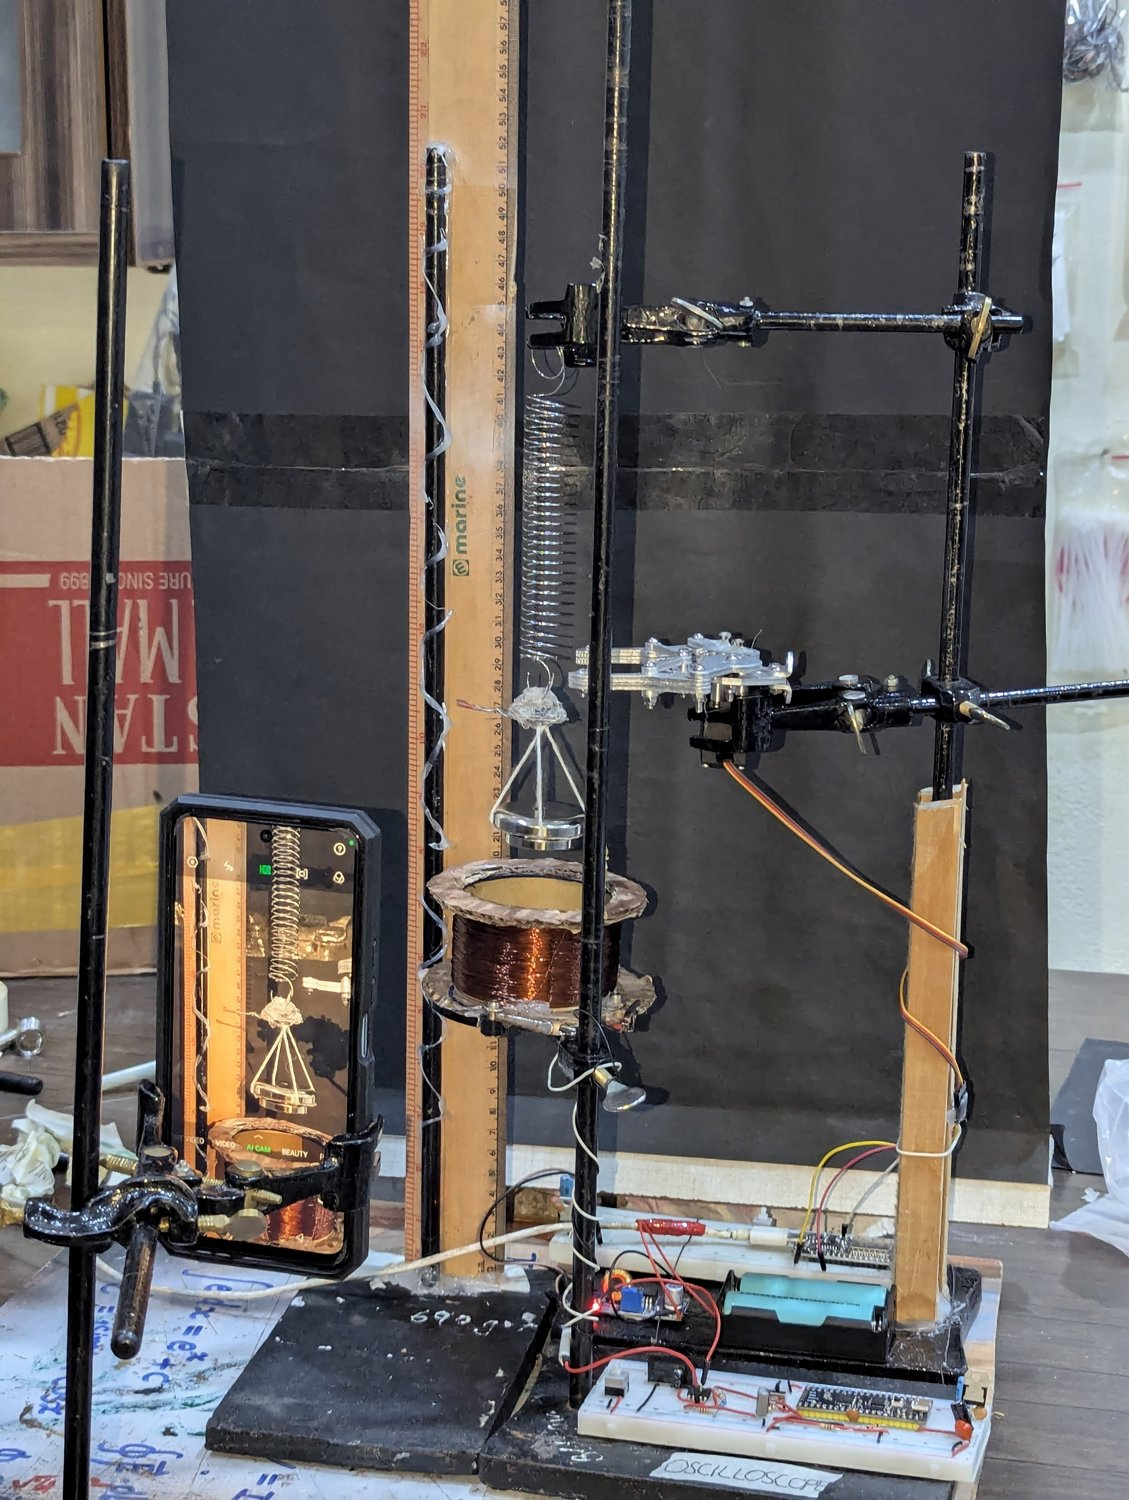
\includegraphics[height=5.3cm]{figs/setup.jpg}\hfill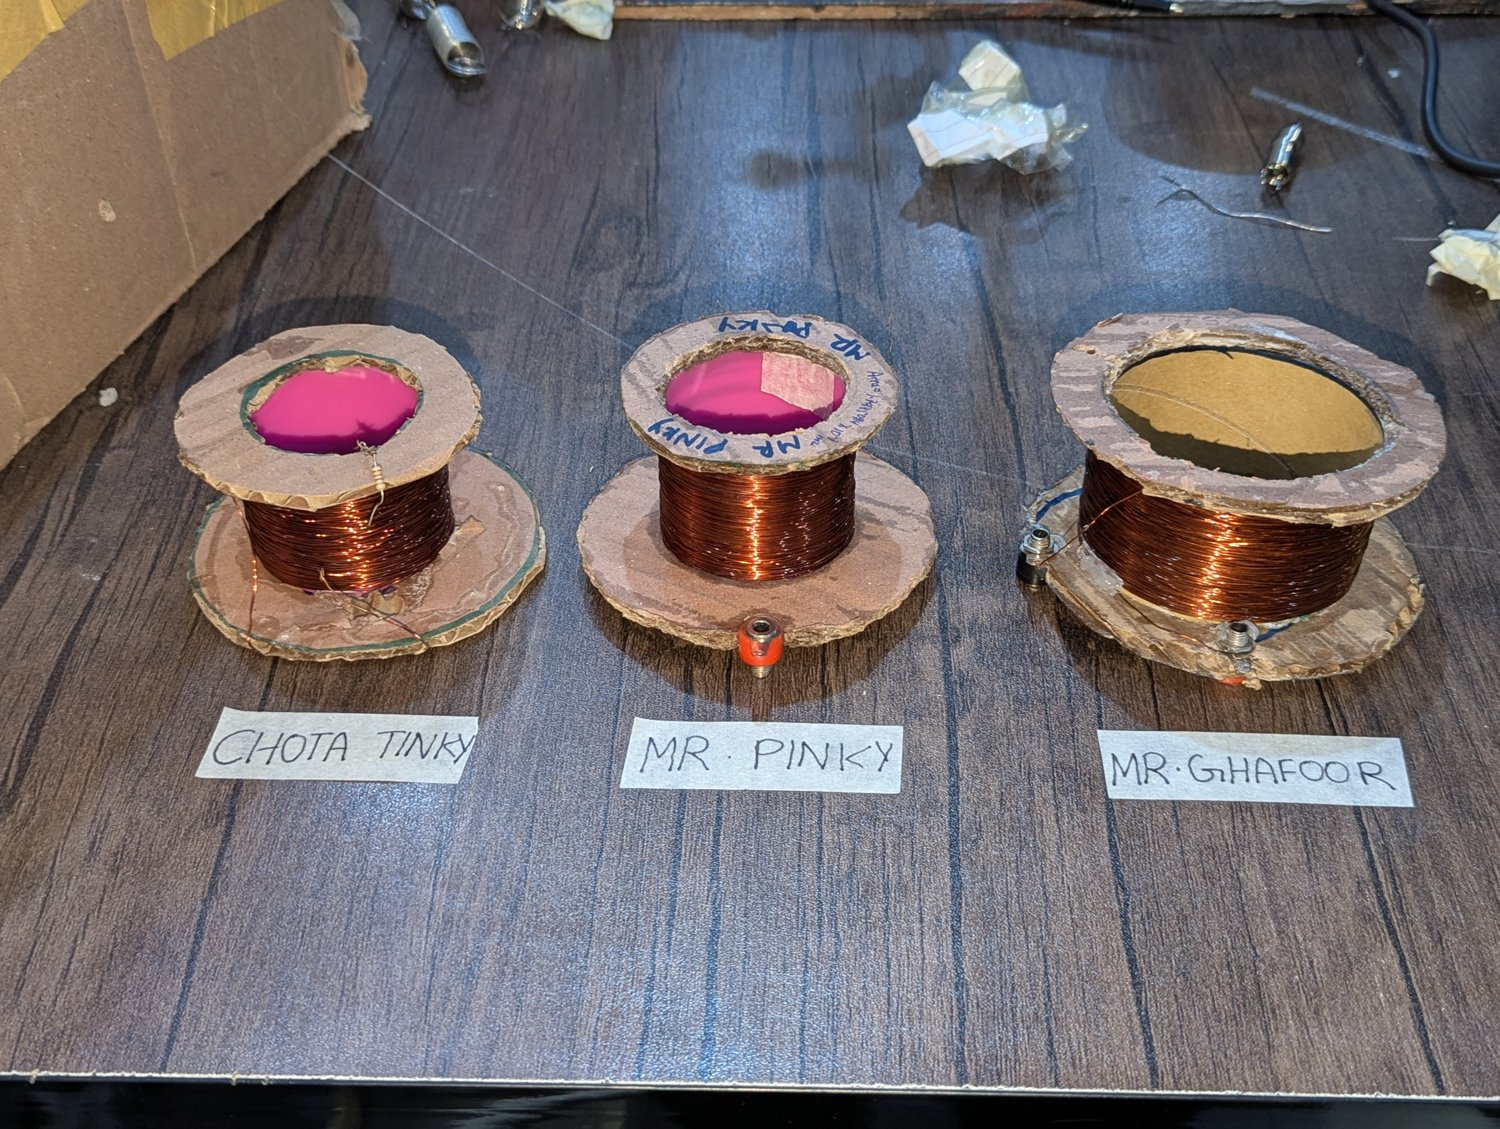
\includegraphics[height=5.3cm]{figs/coils.jpg}\hfill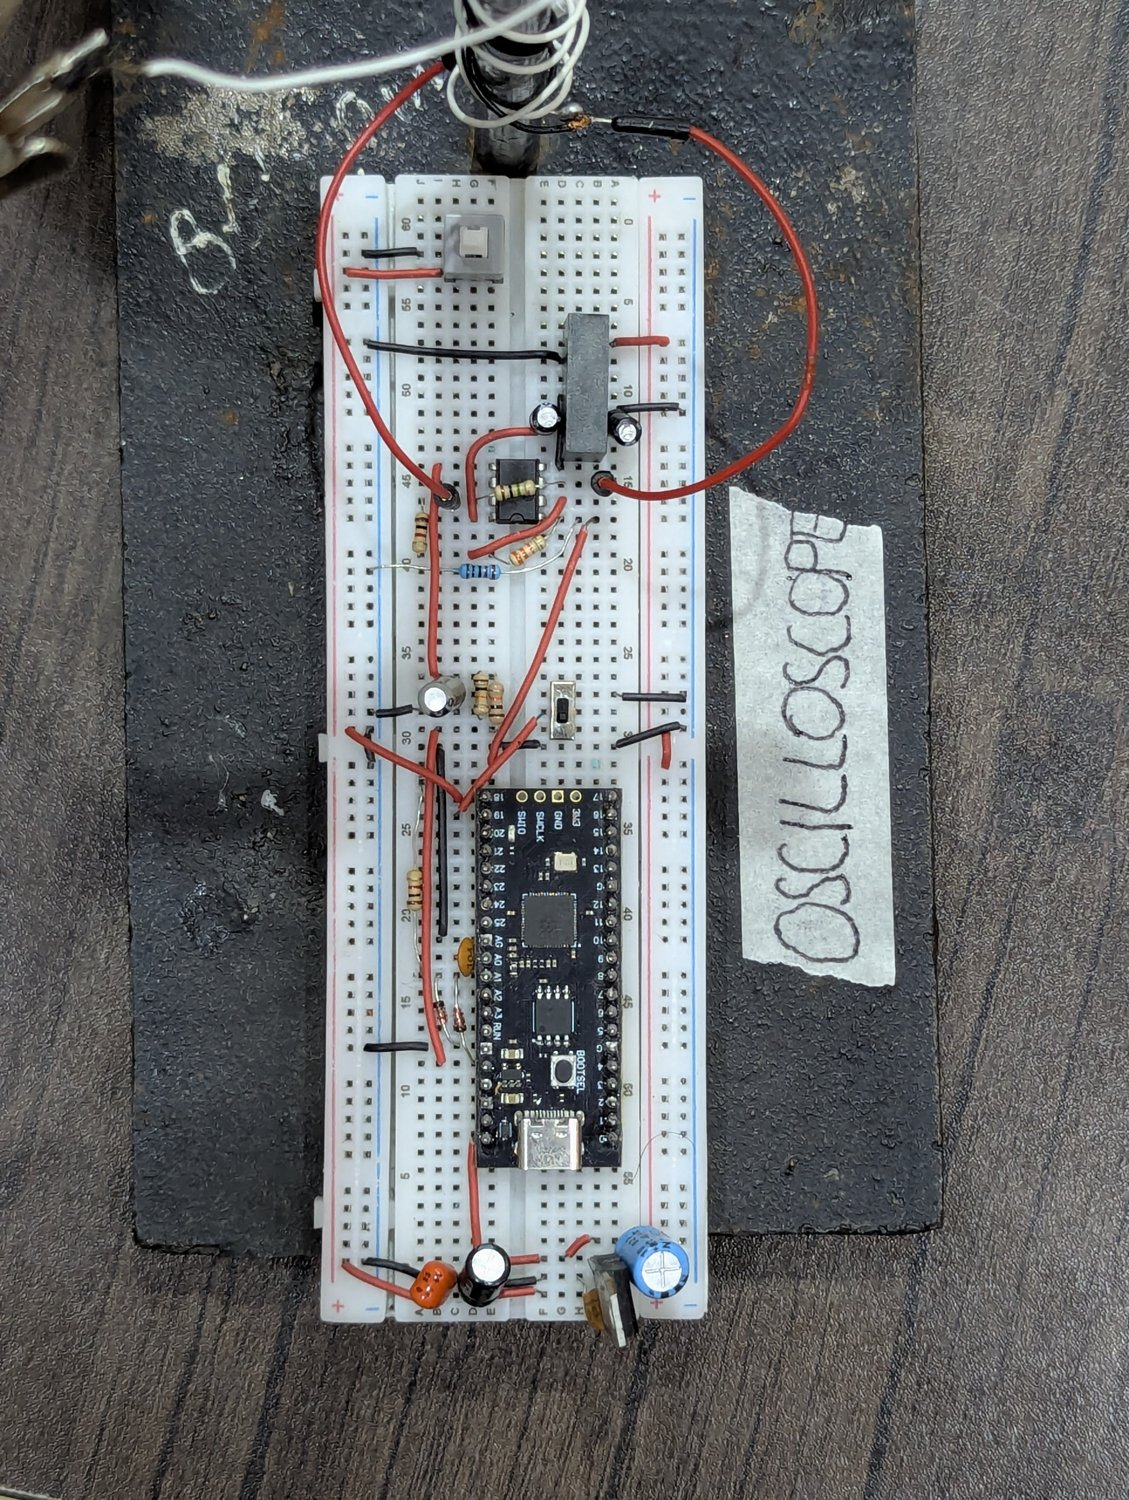
\includegraphics[height=5.3cm]{figs/daq_board.jpg}
\figurenote{Left: the oscillator. The magnets hang in a string cradle from the spring, above coil~1; a servo claw releases the cradle, and a phone records the motion against a metre rule. Note the steel retort rod a few centimetres from the magnet. Centre: the three coils. Right: the breadboard DAQ.}
\end{figure}

\subsection{Data Acquisition}

The coil EMF is tens of millivolts and changes sign, so it cannot go straight into a microcontroller's 0--\SI{3.3}{V} analogue-to-digital converter (ADC). Figure~\ref{fig:chain} shows the signal chain. A buffered divider sets a \SI{1.65}{V} reference, so negative EMF can be represented. The coil drives the high-impedance input of an OPA2134 amplifier (gain 35), whose input is biased to the reference through $R_5 = \SI{1}{\mega\ohm}$. An RC filter (\SI{1.6}{kHz}) and clamp diodes protect the ADC of a Raspberry Pi Pico \parencite{RP2040}. The firmware reads the ADC in a loop, averages blocks of 50 readings, stores up to 60\,000 points in RAM (about \SI{38}{s} at the true spacing) and sends the record over USB after each run. The parts cost US\$43, and the design files, firmware and data are open \parencite{Repo2026}.

\begin{figure}[tbp]
\caption{Signal Chain of the Data-Acquisition System}
\label{fig:chain}
\centering
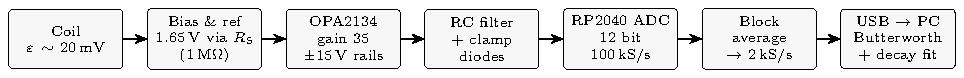
\includegraphics[width=\linewidth]{figs/blocks.pdf}
\end{figure}

The DAQ has several limitations, which we found during this analysis:
\begin{itemize}
\item The block average uses integer division, so each stored value is truncated to one ADC step. The averaging lowers noise but adds no resolution.
\item The recorded step is \SI{23.65}{\micro V} at the input, 2.7\% larger than the repository's firmware constants give. This means the flashed firmware differed slightly from the published version. All EMF values, and hence $c$, carry this 2.7\% scale uncertainty.
\item The input-referred noise before each release ranged from \SIrange{29}{88}{\micro V} rms (median \SI{48}{\micro V}). That is about $3\times10^{-3}$ of the signal.
\item The ADC timestamps are not measured. They are computed as sample number $\times$ \SI{500}{\micro s}. This turned out to be wrong (Lesson~2 below).
\item The op-amp runs from $\pm\SI{15}{V}$ rails. Under overload, the clamps can let the ADC pin exceed its absolute ratings. A single-supply rail-to-rail amplifier with Schottky clamps is safer \parencite{Horowitz2015}.
\end{itemize}

\subsection{Protocol}

With coil~1, an external resistor $R_{\rm ext}$ was placed in series with the coil. It was set to 0, 33.6, 81.4, 324, 1051, 3180 and \SI{9610}{\ohm} for spring~1, with \SI{0}{\ohm} repeated, and to similar values for spring~2. One spring-1 run used \SI{2.2}{\mega\ohm}. Coils~2 and~3 were recorded once on each spring. Each run lasted about \SI{38}{s}, or about 70--80 cycles. A phone filmed every run for video tracking.

\subsection{Analysis}

The analysis scripts are in the repository. Each record was low-pass filtered (fourth-order zero-phase Butterworth, \SI{20}{Hz}; \cite{Virtanen2020}). Because the harmonics in $\varepsilon$ decay faster than the motion does, fitting the EMF peaks overestimates $\gamma$ by about 20\%. Instead, we isolated the fundamental with a band-pass filter at 0.6--1.4~$f$, took its Hilbert envelope (a smooth curve through the oscillation's peaks), and fitted $\ln(\text{envelope})$ against time. The fit started about \SI{1.3}{s} after the first large peak and ended about \SI{1.3}{s} before the end of the record, with one point per cycle. Uncertainties come from a block bootstrap, which refits many resampled versions of each record. Two other estimators of the displacement decay (a nonlinear fit of the fundamental, and a model of the transduction) agree within 7\% (spring~1) and 12\% (spring~2), and we quote their spread as a method uncertainty. Figure~\ref{fig:trace} shows a typical recording and its envelope.

\begin{figure}[tbp]
\caption{A Typical Recording (Spring 1, Coil 1, $R_{\rm ext} = 0$)}
\label{fig:trace}
\centering
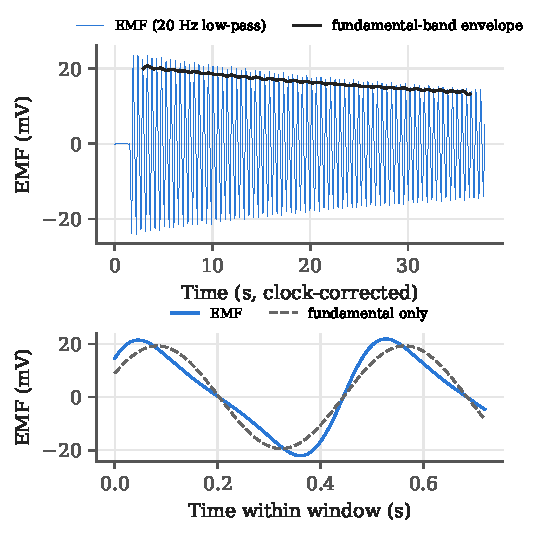
\includegraphics[width=0.62\linewidth]{figs/trace.pdf}
\figurenote{Top: EMF with the envelope of its fundamental. Bottom: the waveform is visibly non-sinusoidal because the coupling $\kappa(z)$ varies along the stroke.}
\end{figure}

\section{Results}

\subsection{The Damping Ignores the Resistance}

Figure~\ref{fig:gR} shows $\gamma$ against $R_c + R_{\rm ext}$. Neither spring shows a trend. Over the eight spring-1 runs below \SI{10}{k\ohm},
\[
\gamma_1 = (11.9 \pm 0.5_{\rm scatter} \pm 0.4_{\rm method} \pm 0.12_{\rm clock})\times10^{-3}\ \mathrm{s^{-1}},\qquad Q_1 = 551 \pm 24 .
\]
For spring~2, $\gamma_2 = (13.5 \pm 1.0)\times10^{-3}\,\mathrm{s^{-1}}$ and $Q_2 = 436 \pm 32$. The \SI{2.2}{\mega\ohm} run, where the circuit is effectively open, gives $\gamma = 11.5\times10^{-3}\,\mathrm{s^{-1}}$, the same as the rest. These values use the corrected timebase described below.

\begin{figure}[tbp]
\caption{Decay Rate Against Coil-Side Series Resistance}
\label{fig:gR}
\centering
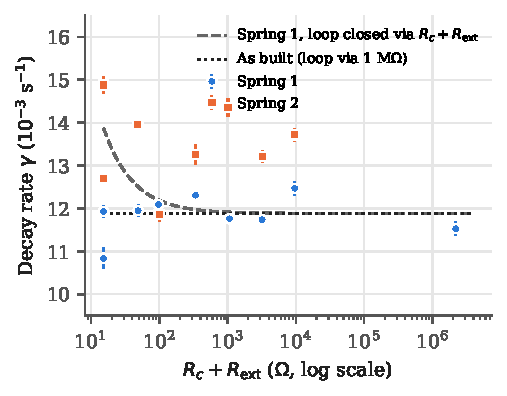
\includegraphics[width=0.62\linewidth]{figs/gamma_vs_R.pdf}
\figurenote{The dashed curve is Equation~\ref{eq:gem} for spring~1 if the loop had been closed through $R_c+R_{\rm ext}$. The dotted line is the prediction for the circuit as built. Error bars are bootstrap standard errors.}
\end{figure}

From the measured EMF ($\varepsilon_{\rm rms} \approx \SI{16}{mV}$ over the first three cycles) and the initial amplitude $A \approx \SI{2.2}{cm}$ seen in the video, Equation~\ref{eq:gem} gives $c = \SI{0.030}{\ohm\,s^{-1}}$. Closed through the coil alone, the loop would therefore have added $\gamma_{\rm em} \approx 2.0\times10^{-3}\,\mathrm{s^{-1}}$, about 17\% of the total (9--25\% for $A$ between 3.0 and \SI{1.8}{cm}). That effect is several times larger than the run-to-run scatter. A fit of $\gamma = \gamma_0 + c/(R_c+R_{\rm ext})$ to spring~1 gives $c = (-0.011 \pm 0.006)\,\Omega\,\mathrm{s^{-1}}$, which disfavours the predicted value by about 3 standard deviations if $A$ is taken as exact, and by 2.3 if $A$ is uncertain by 20\%. A permutation test, which reshuffles the decay rates among the resistances, gives $p = .003$. The fitted $c$ is itself slightly negative, which no physical loss could produce, so the run-to-run scatter is the limiting factor. The decisive argument is the circuit analysis below, not this fit.



\subsection{Lesson 1: The Loop Was Never Closed}

The coil connects between the \SI{1.65}{V} reference and the non-inverting input of the amplifier (Figure~\ref{fig:circuits}a). The only path that closes the coil circuit is $R_5$. Adding $R_{\rm ext}$ in series changed $R_{\rm loop}$ from \SI{1.000}{\mega\ohm} to at most \SI{1.010}{\mega\ohm}. The current was always about $\SI{16}{mV}/\SI{1}{\mega\ohm} \approx \SI{16}{nA}$, dissipating about \SI{0.3}{nW}. The mechanical loss is about \SI{0.1}{mW}. By Equation~\ref{eq:gem}, $\gamma_{\rm em} \approx 3\times10^{-8}\,\mathrm{s^{-1}}$ in every run. The DAQ measured the EMF accurately, but no braking current ever flowed.

Two observations support this diagnosis.
\begin{itemize}
\item \textbf{The \SI{2.2}{\mega\ohm} run.} Here $R_{\rm ext}$ and $R_5$ form a voltage divider, so the recorded EMF should fall to $10^6/(3.2\times10^6) = 0.31$ of its usual value. After correcting for this run's 15\% smaller release, it is 0.30.
\item \textbf{The low resistances.} Small resistors made no measurable difference to the recorded EMF. That confirms they were wired in series with the coil: a \SI{33.6}{\ohm} resistor across the coil would instead have cut the recorded EMF to about 0.69 of its usual value.
\end{itemize}
The \SI{2.2}{\mega\ohm} run also shows the strongest mains pickup, as expected for a high-impedance node.

\begin{figure}[tbp]
\caption{The Circuit as Built and a Corrected Version}
\label{fig:circuits}
\centering
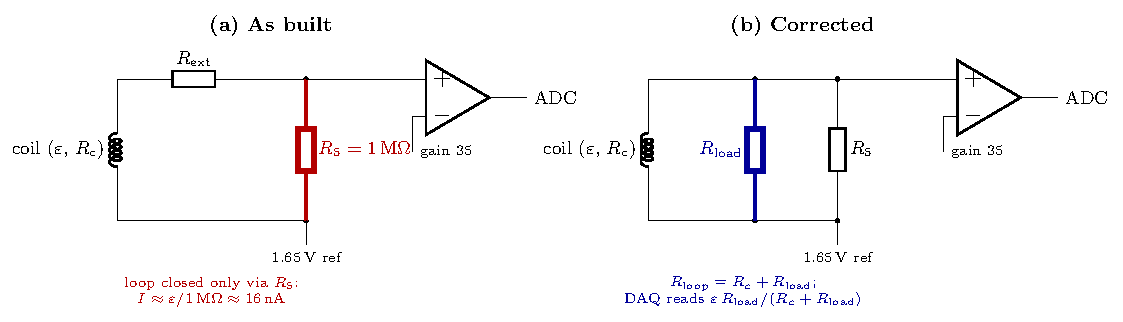
\includegraphics[width=\linewidth]{figs/circuits.pdf}
\figurenote{(a) The coil is closed only through the \SI{1}{\mega\ohm} bias resistor, so almost no current flows. (b) A load resistor across the coil terminals sets $R_{\rm loop} = R_c + R_{\rm load}$. The DAQ then reads $\varepsilon R_{\rm load}/(R_c+R_{\rm load})$.}
\end{figure}

\textbf{A corrected circuit.} The braking current needs a known, low-resistance path. The simplest fix is to put $R_{\rm load}$ directly across the coil, in parallel with the amplifier input (Figure~\ref{fig:circuits}b), and to vary it. Comparing an open coil with a shorted coil gives $\gamma_{\rm em}$ directly. A transimpedance input does better: the coil and $R_{\rm ext}$ feed the inverting input of an op-amp with a feedback resistor. That closes the loop through only $R_c + R_{\rm ext}$, measures the current directly, and lets the original series-resistor protocol work unchanged.

\subsection{Lesson 2: The Clock Was Never Checked}

Every recording contains a narrow line at \SI{63.07 \pm 0.23}{Hz}, with a harmonic at \SI{126.1}{Hz} (Figure~\ref{fig:hum}). Pakistan's mains frequency is \SI{50}{Hz}. If this line is mains pickup, the true spacing between stored samples is $s = 63.07/50 = 1.261 \pm 0.013$ times the spacing the firmware assumed; we call $s$ the clock factor, and its uncertainty is set by the grid's tolerance. Three features identify the line as mains: it has harmonics, it is strongest in the high-impedance \SI{2.2}{\mega\ohm} run, and its frequency wanders by 0.4\% between runs while the spring frequency stays fixed to 0.02\%, as expected for the grid and not for a crystal-timed source such as the servo controller. Lighting flicker would appear at \SI{100}{Hz}. The cause is in the firmware. It schedules each ADC read \SI{10}{\micro s} after the last. When one read plus the loop overhead takes longer, the loop simply runs flat out. Each read then takes about \SI{12.6}{\micro s}, and each stored point is \SI{631}{\micro s} apart, not \SI{500}{\micro s}. A 60\,000-point record therefore lasts \SI{37.9}{s}, not \SI{30}{s}; timing one recording with a stopwatch or video would confirm this directly.

\begin{figure}[tbp]
\caption{Mains Hum as a Clock}
\label{fig:hum}
\centering
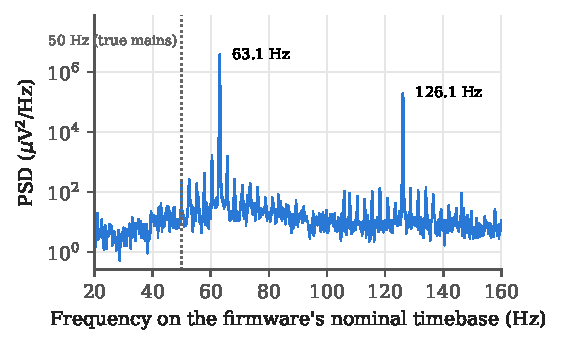
\includegraphics[width=0.62\linewidth]{figs/hum.pdf}
\figurenote{Noise spectrum of the \SI{2.2}{\mega\ohm} run, plotted on the firmware's assumed timebase. The mains line, truly at \SI{50}{Hz}, appears at \SI{63.1}{Hz}.}
\end{figure}

The correction divides every frequency and decay rate by $s$, while leaving $Q$ unchanged. Two independent checks agree with it:
\begin{itemize}
\item \textbf{Video.} The phone video runs on its own clock. The ratio of its decay rates to the DAQ values is $1.06 \pm 0.06$ with the clock correction and $0.84 \pm 0.05$ without it, so the video favours the correction. Because the per-run video rates scatter widely, this checks the overall scale only; counting oscillation cycles in the video would be a much tighter test.
\item \textbf{Spring constants.} The corrected frequencies are \SI{2.08}{Hz} and \SI{1.86}{Hz}. Their ratio, 1.118, does not depend on $s$. It is consistent with the measured spring constants only if the two $k$ labels were interchanged (predicted 1.083). With the labels swapped, both frequencies lie 4--7\% below the static-$k$ predictions. Spring mass lowers the frequency by only about 1\%, and because $k$ came from the slope of a force--extension graph, initial tension in the spring does not bias it. The remaining gap is unexplained; an error in the oscillating mass or in the $k$ measurements is possible. Re-measuring $k$, and timing the DAQ directly, would settle both points; we could not repeat the measurements after the internship.
\end{itemize}

\subsection{The Damping That Remains Is Mechanical}

Since $\gamma_{\rm em}$ was negligible, the measured damping is entirely mechanical, and it is not exponential. The first half of each run decays faster than the second, by $11 \pm 12\%$ for spring~1 (7 of 8 runs) and $19 \pm 6\%$ for spring~2 (all 8 runs). For spring~2, whose release amplitude varied more, $\gamma$ also correlates strongly with the initial EMF ($r = .97$, Figure~\ref{fig:amp}); for spring~1, whose release amplitude varied by only 6\%, there is no such trend ($r = -.40$). The amplitude dependence is therefore clear for spring~2 and weaker for spring~1. Air drag on the cradle is about 2\% of the damping, too small to explain this. Candidates are coupling to the cradle's pendulum or torsional modes \parencite{Berg1991}, friction at the string attachments, and losses in the steel retort rod a few centimetres from the magnet. We cannot yet tell them apart. A control run with the rod moved away would test the last.

\begin{figure}[tbp]
\caption{Decay Rate Against Initial EMF, a Proxy for Release Amplitude}
\label{fig:amp}
\centering
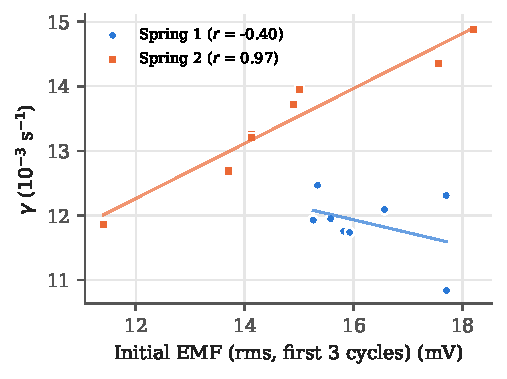
\includegraphics[width=0.6\linewidth]{figs/gamma_vs_amp.pdf}
\end{figure}

The coil geometry changes the EMF but, with no current flowing, not the damping. Coil~2, with a different former diameter, gave 0.37 (spring~1) and 0.45 (spring~2) of coil~1's EMF. Coil~3, with a different wire gauge, gave about 0.11. The decay rates for coils~2 and~3 were the same as for coil~1 within the scatter.

\section{Discussion}

Neither error is exotic. A high-impedance input is the right choice for measuring an EMF and the wrong one for producing braking. A microcontroller loop that cannot keep up with its schedule fails silently. Both errors left clean-looking data: smooth exponential decays and a stable frequency. The first was revealed only because the expected $1/R$ dependence was missing. The second was revealed by the mains line, which we went looking for because the measured frequencies disagreed with the spring constants. The checks below would have caught both in the first hour.

\begin{mdframed}[linewidth=0.6pt,innertopmargin=6pt,innerbottommargin=6pt,nobreak=true]
\textbf{Lessons for Instructors}
\begin{enumerate}
\item Before blaming the physics, compute the current your circuit actually allows, $I = \varepsilon/R_{\rm loop}$.
\item A high-impedance input on a coil measures the EMF but brakes nothing; give the braking current a known low-resistance path.
\item Do not trust a microcontroller's assumed sample rate. The \SI{50}{Hz} (or \SI{60}{Hz}) hum already in your data is a free clock.
\item Before collecting a full data set, run an open-coil versus shorted-coil control and check that the predicted effect exceeds your run-to-run scatter.
\item Compare the early and late halves of each decay; a single exponential fit can hide amplitude-dependent losses.
\end{enumerate}
\end{mdframed}

Our study has limitations. Each resistance was recorded once (twice at \SI{0}{\ohm}). The coil and magnet geometry were not fully documented. The amplitude $A$ in Equation~\ref{eq:gem} comes from video. The clock correction rests on the mains frequency rather than a direct timing measurement. None of these affects the central conclusion: the \SI{1}{\mega\ohm} path cut the current by a factor of $R_5/R_c \approx 7\times10^{4}$ compared with a coil closed on itself.

\section{Conclusion}

A low-cost DAQ recorded millivolt coil EMFs cleanly, yet changing the series resistance from \SI{15}{\ohm} to \SI{2.2}{\mega\ohm} did not change the damping of a magnet--spring oscillator. The coil circuit was closed only through a \SI{1}{\mega\ohm} bias resistor, so the electromagnetic damping was a few millionths of the total. Separately, mains hum showed that the DAQ's sample spacing was 26\% longer than assumed; the correction agrees with video timing and, if two spring labels were swapped, with the spring constants. Both are easy mistakes, easy to detect, and worth teaching.


\section{Acknowledgments}

We thank our supervisors, M. Sanan Qureshi, Dr Sadia Manzoor and Dr Pervez Hoodbhoy, for their guidance, and the staff of The Black Hole Science Lab, including Sayed Iqtidar Ali Shah, for help with the apparatus. This work was carried out within the 2026 Black Hole Science Internship Programme.

H.~T.~Malik led the conceptualization, theory, formal analysis and writing; H.~Kumar wrote analysis software and did the video tracking; M.~U.~Farooq collected the data and maintained the DAQ hardware and firmware. All authors reviewed the manuscript. The authors have no conflicts of interest to disclose.

An AI assistant (Claude, Anthropic) was used to reanalyse the raw data, including the fundamental-band decay estimator and the mains-hum clock calibration, to simulate independent referee reviews, and to edit the manuscript. The authors checked the analysis and text and take full responsibility for the content.

\section{Data and Code Availability}

For transparency and further research, all raw data, the DAQ firmware and schematics, the analysis code that reproduces every number and figure in this paper, and the internal review record are available in the following GitHub repository: \href{https://github.com/smash09x/magnet-spring-em-damping}{github.com/smash09x/magnet-spring-em-damping}.

\printbibliography

\section{Appendix}

\renewcommand{\thetable}{A\arabic{table}}
\setcounter{table}{0}
\begin{table}[h]
\caption{Decay Rate, Quality Factor and Frequency for Every Run}
\label{tab:A1}
\centering\small
\begin{tabular}{@{}llrrrrr@{}}
\toprule
Spring, coil & $R_{\rm ext}$ ($\Omega$) & $\gamma$ ($10^{-3}$ s$^{-1}$) & SE & $Q$ & $f$ (Hz) & $\varepsilon_{\rm rms}$ (mV)\\
\midrule
Spring 1, Coil 1 & 0 (a) & 10.84 & 0.25 & 603 & 2.081 & 17.7\\
 & 0 (b) & 11.93 & 0.14 & 549 & 2.083 & 15.3\\
 & 33.6 & 11.95 & 0.14 & 547 & 2.081 & 15.6\\
 & 81.4 & 12.09 & 0.11 & 541 & 2.082 & 16.6\\
 & 324 & 12.31 & 0.11 & 531 & 2.082 & 17.7\\
 & 1051 & 11.76 & 0.11 & 556 & 2.082 & 15.8\\
 & 3180 & 11.74 & 0.11 & 557 & 2.082 & 15.9\\
 & 9610 & 12.47 & 0.16 & 525 & 2.082 & 15.3\\
 & 2.2 M & 11.53 & 0.16 & 567 & 2.081 & 4.0\\
Spring 2, Coil 1 & 0 (a) & 14.88 & 0.20 & 393 & 1.861 & 18.2\\
 & 0 (b) & 12.69 & 0.12 & 461 & 1.862 & 13.7\\
 & 33.3 & 13.95 & 0.13 & 419 & 1.862 & 15.0\\
 & 84.1 & 11.86 & 0.16 & 493 & 1.863 & 11.4\\
 & 327 & 13.26 & 0.23 & 441 & 1.862 & 14.1\\
 & 997 & 14.35 & 0.21 & 408 & 1.862 & 17.6\\
 & 3190 & 13.21 & 0.14 & 443 & 1.863 & 14.1\\
 & 9670 & 13.72 & 0.15 & 426 & 1.862 & 14.9\\
Spring 1, Coil 2 & 0 & 10.89 & 0.15 & 601 & 2.084 & 5.9\\
Spring 1, Coil 3 & 0 & 11.67 & 0.15 & 561 & 2.084 & 1.9\\
Spring 2, Coil 2 & 0 & 13.69 & 0.22 & 427 & 1.863 & 6.7\\
Spring 2, Coil 3 & 0 & 13.86 & 0.14 & 422 & 1.863 & 1.6\\
\bottomrule
\end{tabular}
\figurenote{All values use the clock-corrected timebase ($s = 1.261$). $\gamma$ is the decay rate of the fundamental-band Hilbert envelope; SE is its block-bootstrap standard error. $\varepsilon_{\rm rms}$ is the rms EMF over the first three cycles. (a) and (b) mark repeated runs at the same resistance. Generated by \texttt{analysis/run\_all.sh} in the repository.}
\end{table}

\end{document}
